\section{Methodology}
\label{sec:methodology}
\begin{figure}[!htbp]
  \centering
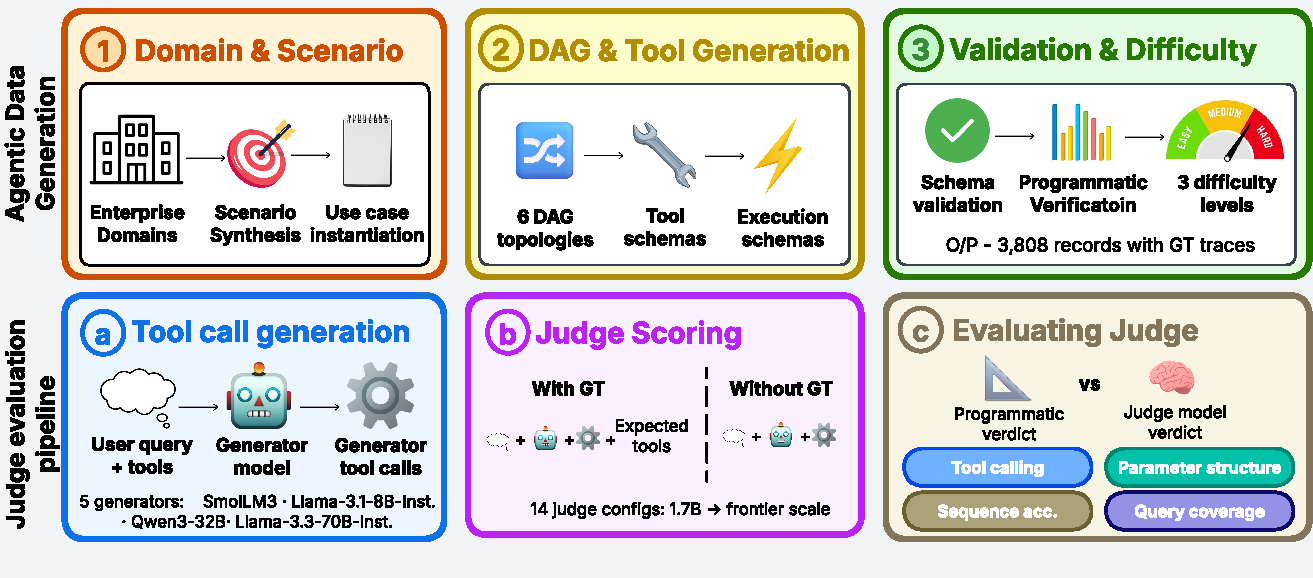
\includegraphics[width=\textwidth]{figures/Judge_Research_Overall_flow}  \caption{%
    Overall pipeline of AgentJudgeBench. Each BFCL-style Agentic record undergoes difficulty-controlled rewriting, generator inference, and parallel scoring by a programmatic judge and LLM judges (with/without GT), followed by alignment with the programmatic reference.%
  }
\label{fig:pipeline}
\end{figure}

Figure~\ref{fig:pipeline} gives an end-to-end view of the pipeline. Each record is expanded into three difficulty variants; every generator $g \in \mathcal{G}$ produces tool-call predictions; a deterministic programmatic judge scores each prediction to yield reference vector $\mathbf{p}_r$; and every LLM judge $j \in \mathcal{J}$ produces paired verdicts $\boldsymbol{\ell}^{\text{GT}}_{j,r}$, $\boldsymbol{\ell}^{\text{no-GT}}_{j,r}$ compared against $\mathbf{p}_r$ via Eq.~\ref{eq:alignment}.

\vspace{-0.1cm}
\subsection{Data Generation}
\label{sec:methodology:data}

The first step of the benchmark (BFCL-style agentic data generation) is constructed through a multi-stage synthetic pipeline that generates complete agentic records from minimal seed inputs, without human-in-the-loop supervision. \\
\textbf{Record construction.} Given an enterprise domain label (e.g., IT Service Management, Contract Lifecycle Management, Energy Grid Operations), the pipeline generates use-case scenarios, synthesizes a typed tool inventory as function signatures with constrained return types (\texttt{str}, \texttt{bool}, \texttt{list}, \texttt{dict}, \texttt{None}), and produces executable pseudocode linking all tool dependencies. A natural language user utterance is then paired with function input/output specifications, and each function is formalized into a JSON schema with typed arguments, required fields, and output definitions. Finally, an ordered execution trace is produced capturing sequential and parallel tool calls, their inputs, outputs, and step descriptions. \\

\textbf{DAG topologies.} Records are organized into six topologies derived from analysis of common dependency patterns in real enterprise agentic workflows: \textit{linear}, \textit{fan-out}, \textit{fan-in}, \textit{diamond}, \textit{optional enrichment}, and \textit{loop-like} - representing progressively complex dependency structures from single-path execution to iterative loops. \\
\textbf{Difficulty tiers.} Each record is expanded into three levels (\textit{easy}, \textit{medium}, \textit{hard}) by increasing query ambiguity while holding the task structure and ground-truth trace constant. Rewrite validation (Appendix~\ref{app:rewrite-validation}) confirms the medium$\to$hard step on $93.9\%$ of records. The easy$\to$medium hardening is unanimously validated on only $58.1\%$ of records; in approximately $41.9\%$ of cases medium is better characterised as a paraphrase rather than a strict difficulty increase. The primary evidence for difficulty-driven degradation is therefore the medium$\to$hard step; medium data should be read as a robustness check rather than a calibrated mid-point (see Limitations, Appendix~\ref{app:limitations}). \\

\begin{wrapfigure}{r}{0.52\textwidth}
  \vspace{-10pt}
  \centering
  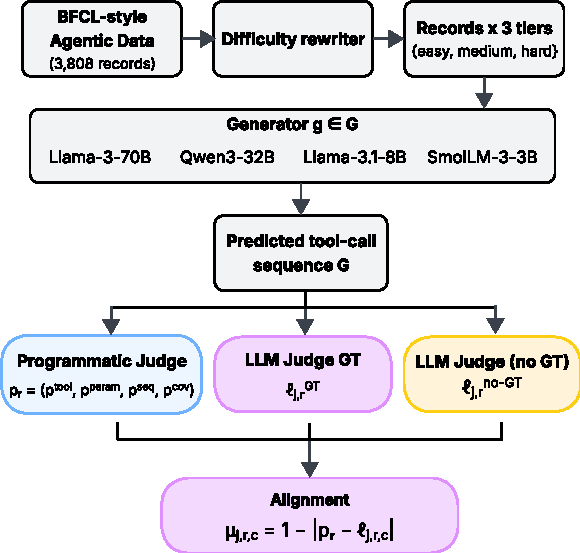
\includegraphics[width=\linewidth]{figures/Evaluator.pdf}
  \caption{Evaluation pipeline of AgentJudgeBench. Records expand into three difficulty tiers, LLM judges (with/without GT) and programmatic judge score the generated tool-call predictions.}
  \label{fig:eval}
  \vspace{-10pt}
\end{wrapfigure}


\textbf{Validation.} Ground-truth traces undergo a two-level quality gate before entering the corpus. First, every record is checked structurally via JSON-schema validation, argument type verification, and programmatic trace consistency checks. Second, each (utterance, tool-call) pair is checked programmatically for argument sufficiency, grounding alignment, and query naturalness; records below threshold are rejected and re-generated. All gate checks are entirely programmatic; no model from $\mathcal{J}$ (or any other LLM) is involved, ruling out self-reinforcing bias in the alignment scores. A 120-record human annotation study on hard-difficulty records (Appendix~\ref{app:prog-judge-validation}), stratified across all six DAG topologies, validates the scorer at $92.7\%$ overall metric-level agreement with independent human judgement (scorer scope and limitations in Appendix~\ref{app:limitations}). The final corpus comprises $3{,}808$ records spanning 15 enterprise domains with 5-14 tools per record, distributed across six topologies and three difficulty levels.


\subsection{Evaluation}
\label{sec:methodology:eval}
As shown in Figure \ref{fig:eval}, our evaluation is layered: a deterministic \emph{programmatic judge} computes a reference score on every record, an \emph{LLM judge} produces a per-metric verdict on the same record, and an \emph{alignment aggregator} compares the two. Each layer is defined below. Symbol definitions appear in Appendix~\ref{app:notation}; all prompts are reproduced verbatim in Appendix~\ref{app:prompts}.

% \vspace{-0.25cm}
\textbf{Programmatic Judge}
\label{sec:methodology:programmatic}

Let $G = (g_1, \dots, g_{|G|})$ denote the generator's predicted ordered sequence of tool calls, and $E = (e_1, \dots, e_{|E|})$ the ground-truth ordered sequence. Let $\mathrm{name}(\cdot)$ return a tool's identifier, $\mathrm{args}(\cdot)$ its argument-key set, and let $\mathcal{G} = \{\mathrm{name}(g_i)\}$, $\mathcal{E} = \{\mathrm{name}(e_i)\}$ denote the unordered sets of tool identifiers. The programmatic judge emits four independent per-record scores in $[0, 1]$.

\paragraph{Tool-selection accuracy $p^{\text{tool}}$ and sequence accuracy $p^{\text{seq}}$.}
$p^{\text{tool}}$ penalises set-level mismatch; $p^{\text{seq}}$ measures position-by-position identity, normalised by expected length:

\begin{subequations}
\begin{minipage}[t]{0.50\linewidth}
\vspace{0pt}
\begin{equation}
p^{\text{tool}} = \max\!\left(0,\, 1 - \frac{|\mathcal{G} \setminus \mathcal{E}| + |\mathcal{E} \setminus \mathcal{G}|}{\max(|\mathcal{E}|, 1)}\right),
\label{eq:prog-tool}
\end{equation}
\end{minipage}%
\hfill
\begin{minipage}[t]{0.46\linewidth}
\vspace{0pt}
\begin{equation}
p^{\text{seq}} = \frac{1}{\max(|E|,1)} \sum_{i=1}^{\min(|G|,|E|)} \mathbb{1}[\mathrm{name}(g_i) = \mathrm{name}(e_i)],
\label{eq:prog-seq}
\end{equation}
\end{minipage}
\end{subequations}

\noindent with $p^{\text{tool}} = p^{\text{seq}} = 1$ when the respective sequences are empty.

\vspace{-0.15cm}
\paragraph{Parameter-structure accuracy $p^{\text{param}}$.}
For each predicted call $g \in G$ let $A_g = \mathrm{args}(g)$ and let $A^{*}_{g}$ be the expected-argument key set of the call in $E$ with the same tool identifier (undefined if the predicted tool is not in $\mathcal{E}$). Define per-call structural scores
\begin{equation}
s(g) \;=\;
\begin{cases}
  1.0 & \text{if } A_g = A^{*}_{g} \ \text{(all required keys present, no extras)} \\
  0.5 & \text{if } A^{*}_{g} \subseteq A_g \ \text{and} \ A_g \setminus A^{*}_{g} \neq \emptyset \ \text{(extras only)} \\
  0.0 & \text{if } A^{*}_{g} \not\subseteq A_g \ \text{or} \ A^{*}_{g} \ \text{undefined},
\end{cases}
\label{eq:prog-param-per-call}
\end{equation}
and aggregate by mean: $p^{\text{param}} = \bigl(\sum_{g \in G} s(g)\bigr) / \max(|G|, 1)$, with $p^{\text{param}} = 1$ when $G$ is empty.

\vspace{-0.25cm}
\paragraph{Query-coverage accuracy $p^{\text{cov}}$.}
Fraction of expected tool identifiers covered by the prediction, ignoring extras:
\begin{equation}
p^{\text{cov}} \;=\;
\begin{cases}
  1                                        & \text{if } \mathcal{E} = \emptyset, \\
  0                                        & \text{if } \mathcal{G} \cap \mathcal{E} = \emptyset, \\
  \lvert \mathcal{G} \cap \mathcal{E} \rvert / \lvert \mathcal{E} \rvert & \text{otherwise}.
\end{cases}
\label{eq:prog-cov}
\end{equation}

\vspace{-0.25cm}
\paragraph{Record-level aggregate.}
Each record receives a four-element programmatic vector $\mathbf{p}_r = (p^{\text{tool}}_r, p^{\text{param}}_r, p^{\text{seq}}_r, p^{\text{cov}}_r)$. Where a scalar is needed - specifically in the generator-accuracy reporting of Table \ref{fig:full-results} - we use the unweighted mean $\bar{p}_r = \tfrac{1}{4} \sum_m p^m_r$; elsewhere the four components are kept separate and averaged independently. We adopt equal weights because the four metrics target orthogonal aspects of tool-call correctness and we have no principled basis for preferring one over another when reporting a single headline number; Section \ref{sec:exp:main} presents per-metric breakdowns that practitioners can reweight for a given application (e.g., upweighting sequence accuracy when judging workflows with strict ordering constraints). Empirically, the judge ranking is stable under alternative metric weightings: Spearman $\rho \geq 0.83$ between the equal-weight ranking and five alternative schemes (seq${\times}2$, param${\times}2$, cov${\times}0.5$, seq${\times}2{+}$param${\times}2$), confirming that the equal-weight aggregate is an adequate proxy for any practitioner-specific weighting.

\textbf{LLM Judge}
\label{sec:methodology:llmjudge}

The same generator outputs scored by the programmatic judge are independently evaluated by every LLM judge $j \in \mathcal{J}$. Each judge receives a structured prompt containing the original user query, the full set of available tool schemas, and the generator's predicted tool-call sequence. The judge is asked to produce a single JSON object scoring each of the four metrics (tool selection, parameter structure, sequence accuracy, query coverage) on a $\{0, 0.5, 1\}$ scale, along with a one-sentence justification per metric and an overall assessment. \\
Two prompt variants exist, corresponding to the conditions $c \in \{\text{GT}, \text{no-GT}\}$: the \textbf{with-GT} prompt additionally exposes the ground-truth tool-call sequence as a reference block, while the \textbf{no-GT} prompt omits it entirely, requiring the judge to assess correctness from the query and tool schemas alone. Judge decoding is held constant across all $(g, j, d, c)$ configurations to isolate the effect of our independent variables. The full prompt bodies appear in Appendix~\ref{app:prompts}.

\textbf{Alignment Against the Programmatic Reference}
\label{sec:methodology:alignment}

Given a record $r$, condition $c$, judge $j$, and metric $m \in \{\text{tool}, \text{param}, \text{seq}, \text{cov}\}$, let $\ell^{m}_{j,r,c} \in \{0, 0.5, 1\}$ denote the judge's verdict and $p^{m}_r$ the programmatic value. The per-metric match score and record-level aggregate are:

\begin{subequations}
\begin{minipage}[t]{0.46\linewidth}
\vspace{0pt}
\begin{equation}
\mu^{m}_{j,r,c} \;=\; 1 - \lvert p^{m}_r - \ell^{m}_{j,r,c} \rvert,
\label{eq:per-metric-match}
\end{equation}
\end{minipage}%
\hfill
\begin{minipage}[t]{0.46\linewidth}
\vspace{0pt}
\begin{equation}
\mu_{j,r,c} \;=\; \tfrac{1}{4} \sum_{m} \mu^{m}_{j,r,c},
\label{eq:overall_alignment}
\end{equation}
\end{minipage}
\end{subequations}

\noindent so that an exact match on all metrics yields $\mu = 1$ and a maximally divergent verdict yields $0$. The configuration-level alignment percentage and ground-truth lift are:

\begin{subequations}
\begin{minipage}[t]{0.54\linewidth}
\vspace{0pt}
\begin{equation}
\mathrm{align}(j, g, d, c) \;=\; \frac{100}{N_{g,d}} \sum_{r=1}^{N_{g,d}} \mu_{j,r,c},
\label{eq:alignment}
\end{equation}
\end{minipage}%
\hfill
\begin{minipage}[t]{0.42\linewidth}
\vspace{0pt}
\begin{equation}
\mathrm{lift}(j) \;=\; \overline{\mathrm{align}}_{\text{GT}}(j) - \overline{\mathrm{align}}_{\text{no-GT}}(j),
\label{eq:lift}
\end{equation}
\end{minipage}
\end{subequations}

\noindent where the overline denotes the mean over all 12 $(g, d)$ configurations. A judge whose verdicts perfectly reproduce the programmatic vector attains $\mathrm{align} = 100\%$; an independent judge attains $50\%$ in expectation. \\
In the experiments that follow, we report both the aggregate alignment $\mathrm{align}(j, g, d, c)$ and per-metric breakdowns to identify which dimensions of tool-calling correctness judges find most difficult to assess.
